\chapter{Implementation}

The implementation of the box model, according to the plans discussed in the previous chapter, mostly went without issues and was able to be put into practice. This chapter presents the steps of implementation taken in detail.

\section{Floor plan}

\begin{figure}[!ht]
    \centering
    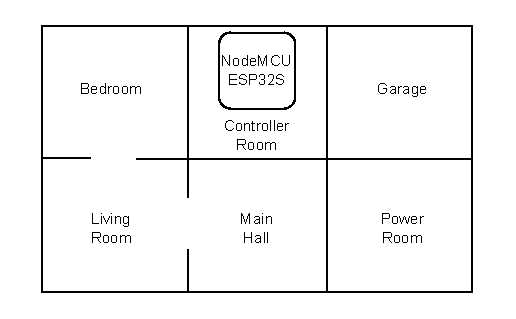
\includegraphics[page=1,keepaspectratio,width=110mm]{figures/box_floorplan.drawio.pdf}
    \caption{Floor plan of the finished box model}
    \label{fig:BoxFloorplan}
\end{figure}

The shoebox used as a base for the project was structured with cardboard and scotch tape to have six equal-sized rooms inside it, shown on \refstruc{fig:BoxFloorplan}. Internal and external cutouts were made in the box to be able to push cables through them, have ventilation holes for the fans, and have a window for the rolling shutter visible from outside.

\section{Connecting devices to the microcontroller}

\begin{figure}[!ht]
    \centering
    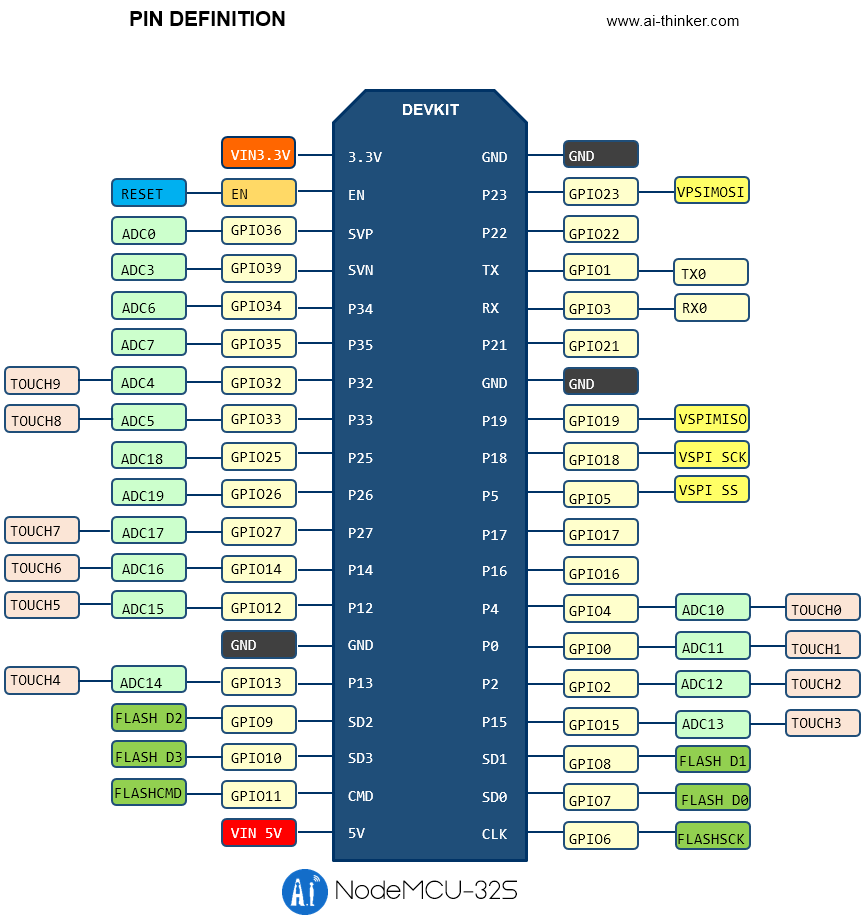
\includegraphics[width=150mm, keepaspectratio]{figures/nodemcu_32s_pinout.png}
    \caption{NodeMCU ESP32S Pinout}
    \label{fig:NodeMCU32Pinout}
\end{figure}

The NodeMCU ESP32S has many ports with different functionalities, as shown on \refstruc{fig:NodeMCU32Pinout}. \cite{AIThinkerNodeMCU32} It has a Micro-USB port that can be used for supplying power and connection to a computer for programming, flashing firmware and serial console. The 5V supplied from the USB port is connected to the VIN 5V pin and there is also a VIN 3.3V port from a voltage converter for supplying power to lower-voltage external components, besides the three ground (GND) pins. There are many more GPIO (General-Purpose Input/Output) pins with different input-output functionalities, however not every of them can be used for every purpose. For example, ADC/DAC pins can be used for Analog-Digital Conversion or vice-versa, therefore sense or create voltages between 0V and 3.3V, some can output PWM (Pulse Width Modulation) signals for dimming LEDs, controlling servos etc., serial pins can be used for serial communication, SD card interfacing and there are some only binary input-output pins. The 3.3V, 5V and ground pins were connected via short bendable solid cables to the power rail sides of the main breadboard for easy distribution of power to components. Jumper cables and wires were used to connect most components to the breadboards, which also served as extension to have appropriate length of cables for them and to be able to put into their desired location inside the box. The method for cable splicing varied, for some, soldering and shrink tubes were used and for others, only wire twisting and electrical tape was used due to the smoke detection system installed in the dormitory, where the project was mostly made.

\begin{figure}[!ht]
    \centering
    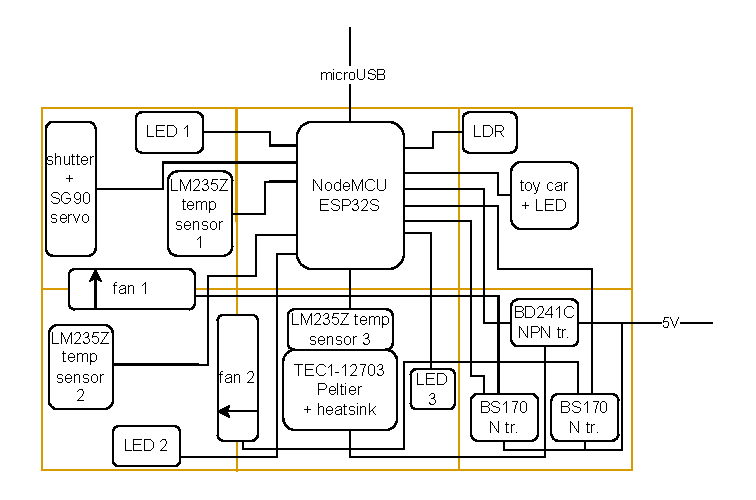
\includegraphics[page=1,keepaspectratio,width=150mm]{figures/box_block_diag.drawio.pdf}
    \caption{Simplified block diagram of components and their wirings inside the box}
    \label{fig:BoxBlockDiag}
\end{figure}

\begin{figure}[!ht]
    \centering
    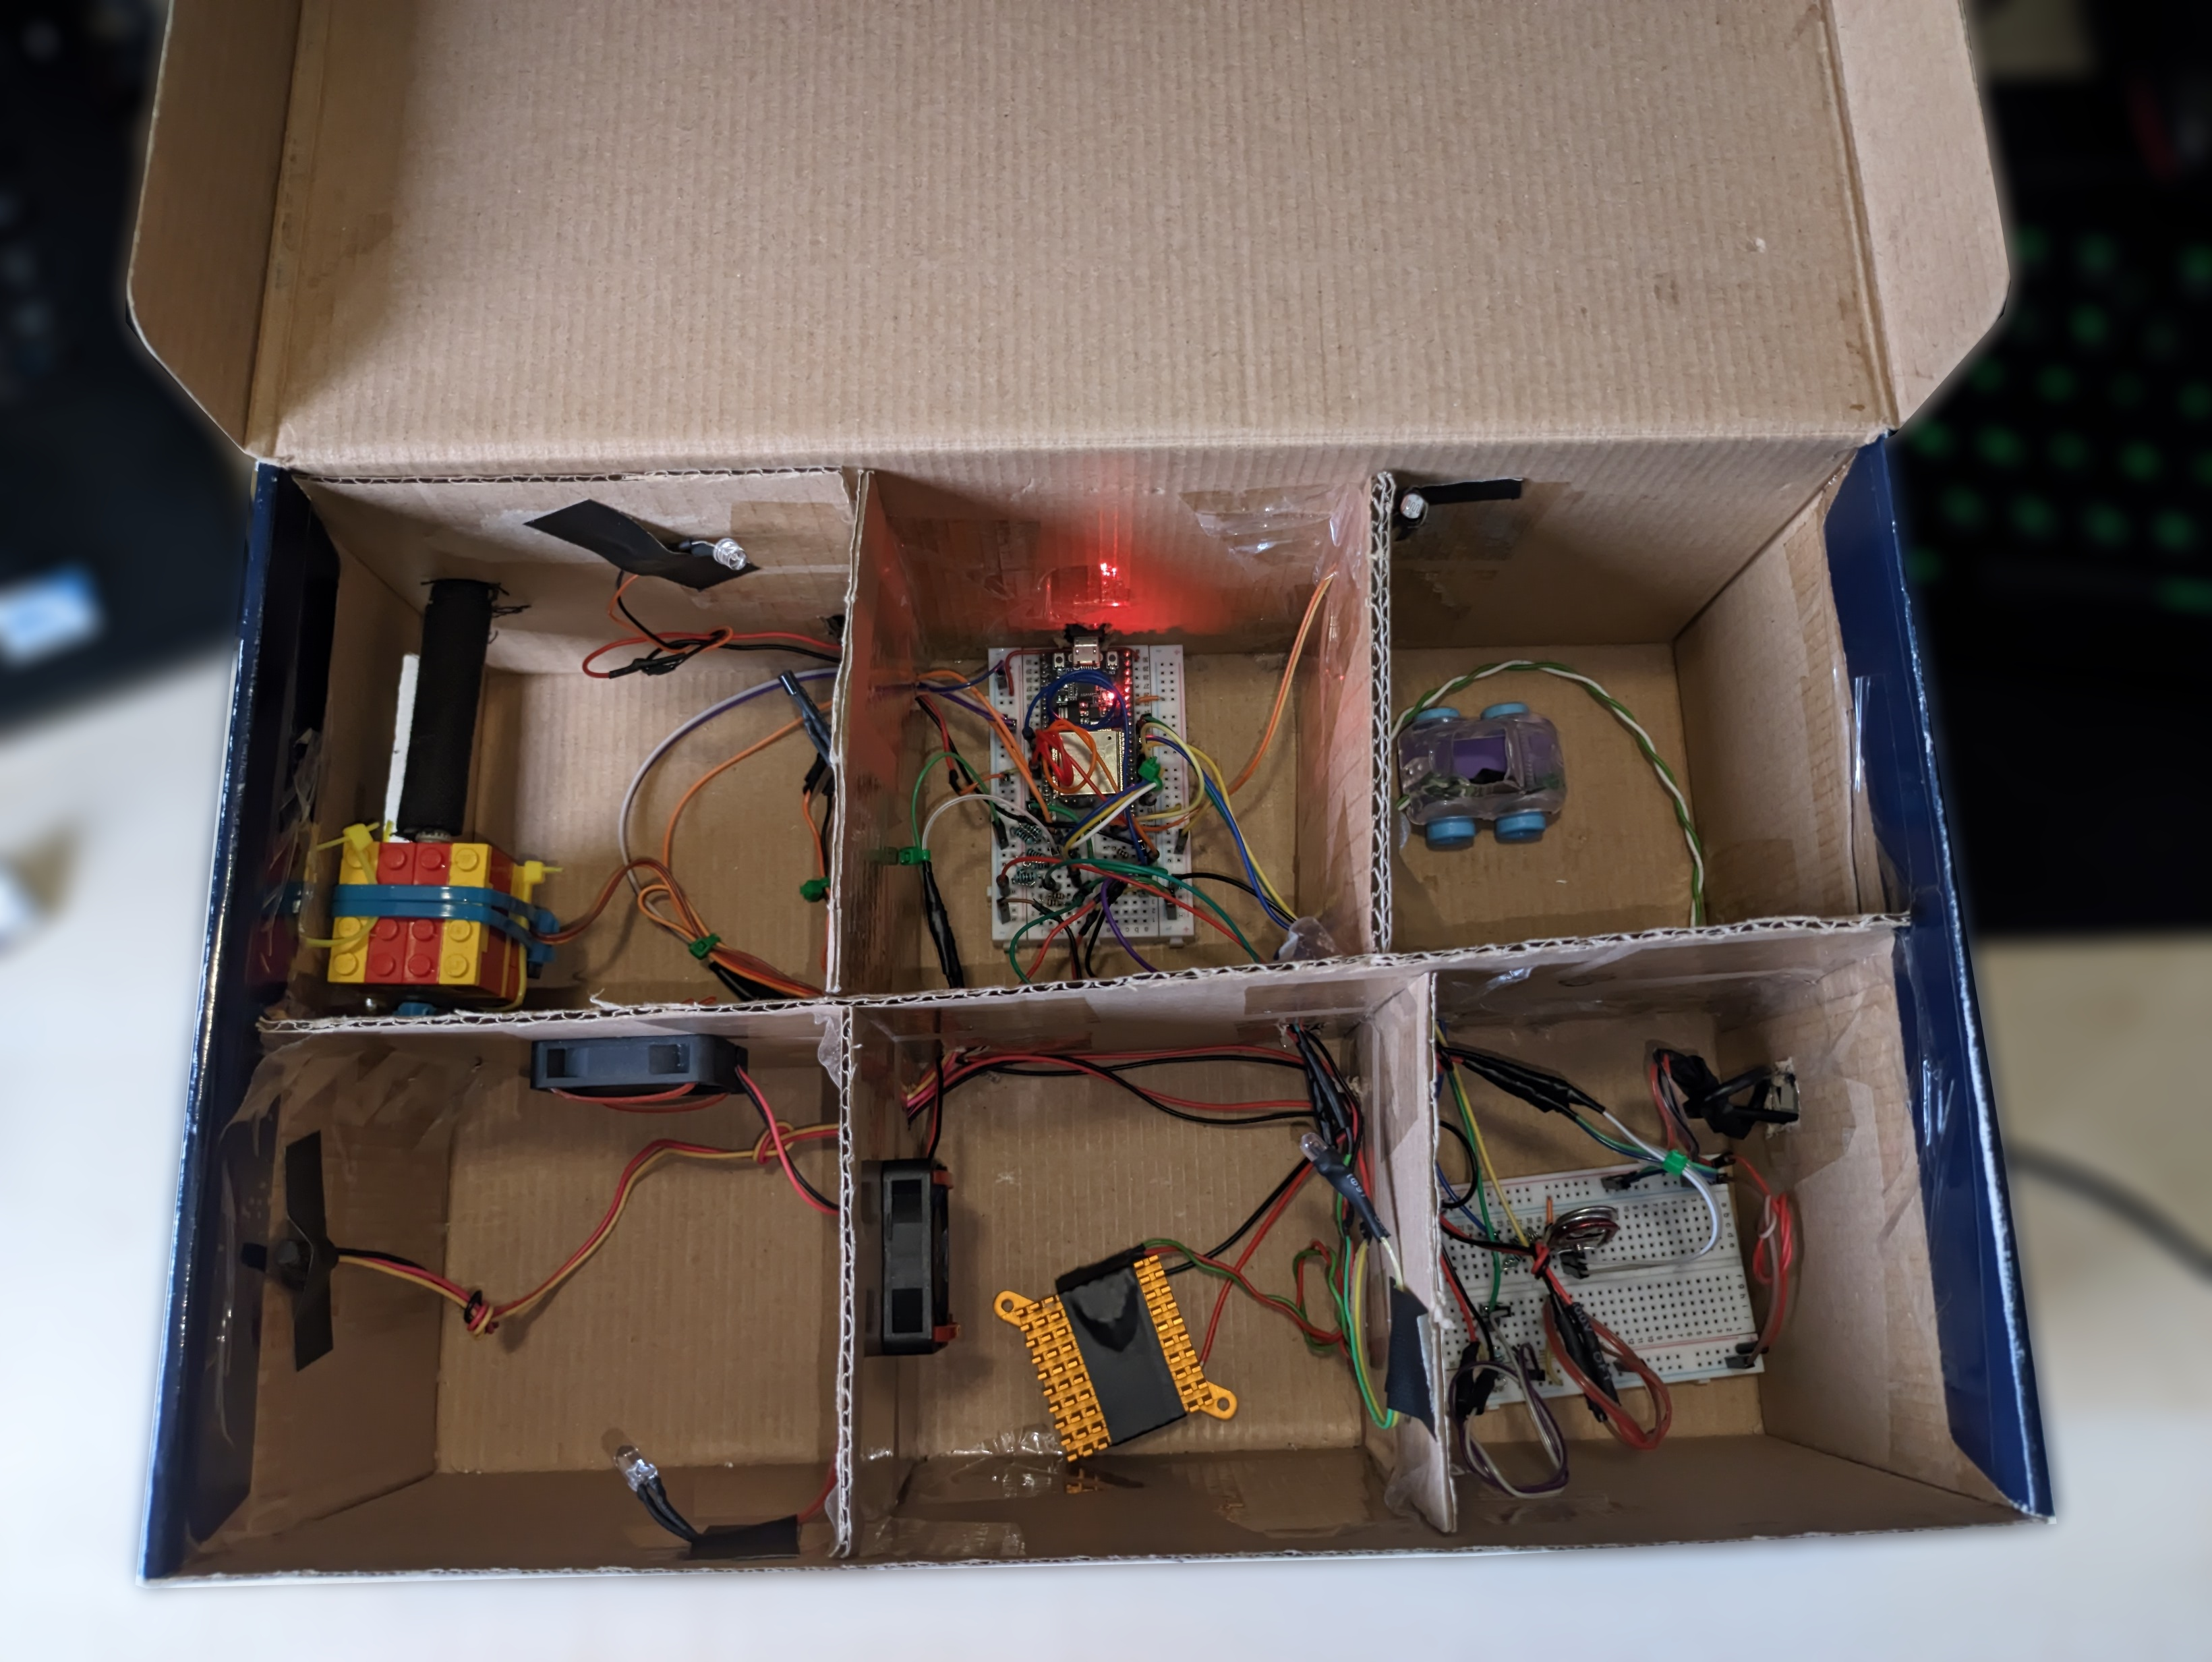
\includegraphics[width=150mm, keepaspectratio]{figures/box_photo.jpg}
    \caption{Photo of the finished box model}
    \label{fig:BoxPhoto}
\end{figure}

The microcontroller's number of pins and their functionalities were adequate the project, extra components can be added up to the limit the available free pins and the required features on them. The pins used for room LEDs were chosen to be non-ADC GPIO pins and for each one, 100$\Omega$ resistors were put between the LED's anode and the microcontroller pin, the cathode was connected to the side ground rail of the breadboard. An LED put inside a small toy car was also connected to a PWM-capable pin with 50$\Omega$ resistance in series to indicate a simulated electric car charging, based on the readings of the light dependent resistor (LDR). The LDR's wiring required a different approach: one end connected to the 3.3V rail, and the other to one of the microcontroller's ADC pins, and to the ground with a 10k$\Omega$ resistor. The three LM235Z temperature sensors were connected with yet another wiring method: 2k$\Omega$ resistors were put between 5V and their V+ terminals, to this the ADC pins were also connected and finally, the V- pins were connected to ground. The SG90 servo was connected to 5V, ground and a PWM capable pin for control. Due to the limited space remaining on the first breadboard, a second one was utilized for the fan and Peltier powering circuit. The ground between the two breadboards was connected with a jumper cable, and a USB cable with male jumper plugs spliced was created to utilize external power from a 5V 2A phone charger. The 5V fans are powered and speed controlled by BS170 transistors utilizing pulse width modulation (PWM). PWM-capable pins of the microcontroller were connected to the transistor's gate terminal, along with 10k$\Omega$ resistors to ground, the source terminal connected to ground and diodes placed between 5V and drain to protect the microcontroller from the inductive load of fans by only allowing flow of electricity in one way. The fans' negative terminals were connected to the transistors' drain and the positive to 5V. Finally, the TEC1-12703 Peltier module has a small heatsink taped onto it and is powered and controlled by a BD241C transistor (with extra cooling attached in the form of soda can tab openers screwed into it for more surface area). This Peltier module's maximum operating voltage is rated to be 15.4V, which means, when run at a lower voltage, it draws less current, therefore functions with a lower power. According to its datasheet, at 5V (which is given by the USB charger), its current is approximately 0.8A, therefore the device draws about 4 watts of power and it decreases with more ambient temperature as the current gets less. \cite{PeltierDatasheet} 333$\Omega$ resistance was used between one of the DAC pins and the transistor's base, the emittor was connected to ground and the Peltier's terminals were connected to the collector and 5V. In \refstruc{fig:BoxBlockDiag}, a simplified block diagram of components and their wirings inside the box is shown without resistors, ground connections, exact pinout of components, and on \refstruc{fig:BoxPhoto}, a photo of the finished box model is shown with the microcontroller turned on.

\section{Network setup}

The Wi-Fi communication medium was set up using a TP-Link WR841N combined network device, targeted for small or home office use. Such devices almost always feature a web-based user interface for their setup and configuration. This was used to flash DD-WRT on it, which is an open-source Linux-based router firmware targeting a variety of Wi-Fi routers and embedded systems. \cite{DDWRTHomepage} It was then set up to mimic a typical home environment, with an SSID of esp\_smart\_home, WPA2-PSK authentication, without internet connectivity and without NAT (Network Address Translation, by setting the operation mode from gateway to router). The IP address range remained the default 192.168.1.0/24 and the router's IP also remained the initial 192.168.1.1, due to it not colliding with other networks actively used on the laptop and smartphone.

An extra Realtek chip based USB Wi-Fi adapter at hand was used for connecting the laptop to the Wi-Fi network, with a custom network profile configuration. Initially, the use of this adapter was done with a network profile limited to the specific network adapter and manual IP configuration was used instead of DHCP to ensure a fixed IP address of 192.168.1.100 and no default gateway learned from this network. Later, it was passed through as a USB device to a virtual machine (VM) with the same Wi-Fi and IP configuration. The Android-based smartphone used for the project was also connected to this network, but didn't have internet connection despite having an Internet-capable SIM card put into it meant as a fallback connection, according to the gained experience.

\section{Software setup}

The chosen software environment discussed in the planning phase was suitable for the usage of obtained hardware, this section showcases the steps taken for its software setup. The personal laptop used for development had a Linux distribution installed, the smartphone used for testing ran Android 14.

\subsection{Home Assistant initial setup, migration}

Initially, Home Assistant was set up in a Docker container environment running on the laptop, with a Docker Compose file specifying the parameters for the container. Docker Engine is a container runtime engine, that makes it possible to run prepackaged container images utilizing the host machine's kernel with minimal overhead and adequate isolation. \cite{DockerContainer} The container images contain a Linux operating system's system libraries, executables and the application itself, therefore provide an easily reproducible, uniform runtime environment despite the differences in various systems. By itself, Docker has a command line interface to run and manage its containers, which means it has to be parameterized from the command line, or put into a script in its parameterized form and executed. Docker Compose is a solution for defining and running multiple Docker containers using an easy-to-manage definition, put into a YAML file. \cite{DockerCompose} YAML is a human-friendly data serialization language with a really simple syntax, as shown in listing \ref{lst:YAMLexample}. \cite{YAMLHomepage}

\begin{lstlisting}[language=,caption=YAML file example,label=lst:YAMLexample]
  shopping_list:
    - bread
    - milk
    - chocolate

  # ideal room temperature
  temperature: 22

  winter_months: ["December", "January", "February"]
\end{lstlisting}

In listing \ref{lst:HADockerCompose}, the Docker Compose definition of the set up Home Assistant container can be seen: 2024.10.3 is the selected version (tag) of the image is used, the config directory from the compose file's directory is mounted directly into the container's file system as /config along with the host machine's local time and dbus for time and device access, and finally, socket connections are bound on the host machine's 8123 port on the Wi-Fi card and localhost interfaces to access the same port inside the container.\break

\begin{lstlisting}[language=,caption=Docker Compose file used for the initial Home Assistant environment,label=lst:HADockerCompose]
services:
  homeassistant:
    container_name: homeassistant
    image: "ghcr.io/home-assistant/home-assistant:2024.10.3"
    volumes:
      - ./config:/config
      - /etc/localtime:/etc/localtime:ro
      - /run/dbus:/run/dbus:ro
    ports:
      - 192.168.1.100:8123:8123
      - 127.0.0.1:8123:8123
\end{lstlisting}

Even though only one container is defined in the compose file, it still shows Compose's advantage, as the environment can be run with a simple command in the terminal, when inside the compose file's directory:

\begin{lstlisting}[language=]
docker compose up
\end{lstlisting}

This setup in the Docker environment functioned properly, however had one limitation: Home Assistant add-ons aren't supported in the container variant, only in the Home Assistant Operating System (HA OS) or the Supervised installation (installed on top of a Linux installation) variants. \cite{HAaddons} A voice assistant was a sought after feature in the project, therefore it was migrated to the HA OS variant, run inside a virtual machine, or VM.

Virtual machine hypervisors allow physical, or host computer resources to be shared to multiple virtual machines, or guest machines. \cite{VMwareVM} Each virtual machine can run it's own separately with its own amount of CPU cores, RAM, storage and other kinds of resources. Virtual Machines are widely used today in IT infrastructures, as the technology makes it easier to create heterogeneous software environments and can offer less downtime with clustered servers. The most popular current virtualization solutions include VMware products, Oracle VirtualBox and Proxmox. \cite{G2freeVM}

\begin{figure}[!ht]
  \centering
  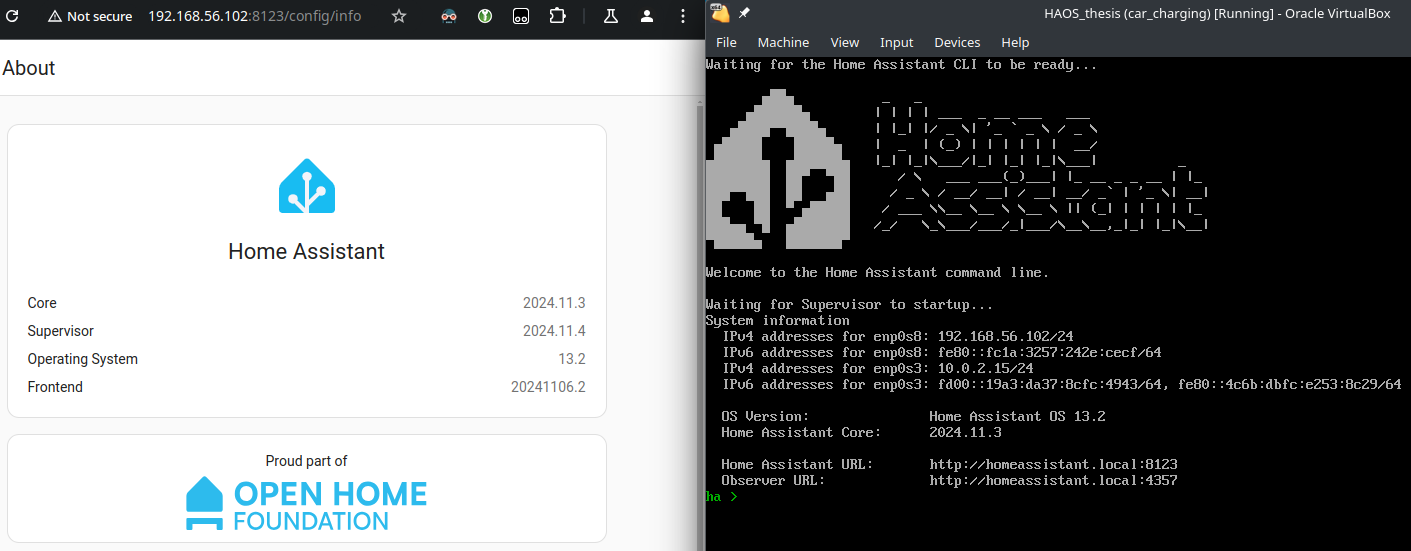
\includegraphics[width=150mm, keepaspectratio]{figures/homeassistant_about.png}
  \caption{Home Assistant OS running in VirtualBox with its web GUI opened from a browser}
  \label{fig:HAabout}
\end{figure}

To run HA OS, the selected VM hypervisor solution was Oracle VirtualBox, due to it being free and and the previous experience gained with it in the past. HA OS is distributed in different disk file formats for various hypervisors, VDI was used for VirtualBox.
Initially, 2 virtual CPU cores and 2 GB of RAM of the host's 16 GB was assigned to it, however it was later changed to 4 GB of RAM to run the voice assistant functionality faster. Two virtual network adapters were added to the VM: one in NAT mode, to provide Internet connection for updates and downloading add-ons, and one adapter in Host-only adapter mode, to be able to be reached from the host (on it's web UI (8123) and SSH (22) ports). Most VM hypervisors offer USB passthrough to virtual machines, which hides the USB device from the host and makes it seem as it was connected to the VM directly. USB passthrough was used to access the USB Wi-Fi adapter inside the VM and the network credentials were set via a parameterized \verb+ha network+ command with the specific SSID, password and IP configuration. The SSH addon was also installed to access command line configurations from a client terminal installed on the host operating system. The configuration of the new environment (eg. integration and dashboard setups) didn't needed to be redone from scratch, as the old environment could be exported to a tar backup file, which was then able to be imported to the new HA OS environment without issues during its initial setup from the web GUI.

\subsection{ESPHome}

To get started with installing ESPHome on the microcontroller, its official getting started with command line guide was followed. \cite{ESPHomeGettingStarted} A sample configuration YAML file was created using the wizard command. The ESPHome compiler and flasher was run from a Docker environment, first flashed via USB and later updated wirelessly using ESPHome's the Over-the-Air (OTA) functionality via Wi-Fi.

\begin{lstlisting}[language=,caption=Docker command to compile and flash ESPHome via OTA / USB,label=lst:ESPHomeDocker]
# for first flashing, add: --device=/dev/ttyUSB0
docker run --rm -v "./esphome":/config -it ghcr.io/esphome/esphome:2024.11.1 run smarthome.yaml
\end{lstlisting}

By default, an ESPHome configuration file only consists of one main YAML file, which contains all configurations. On listing \ref{lst:ESPHomeWizardEx}, an excerpt of a configuration file is shown generated by the wizard for the NodeMCU ESP32S microcontroller.

\begin{lstlisting}[language=,caption=Excerpt of a configuration file generated by the ESPHome wizard,label=lst:ESPHomeWizardEx]
esphome:
  name: livingroom
esp32:
  board: nodemcu-32s
  framework:
    type: arduino
ota:
  - platform: esphome
    password: ""
wifi:
  ssid: "homenetwork"
  password: "teriyaki-noodles"
\end{lstlisting}

\begin{figure}[!ht]
  \centering
  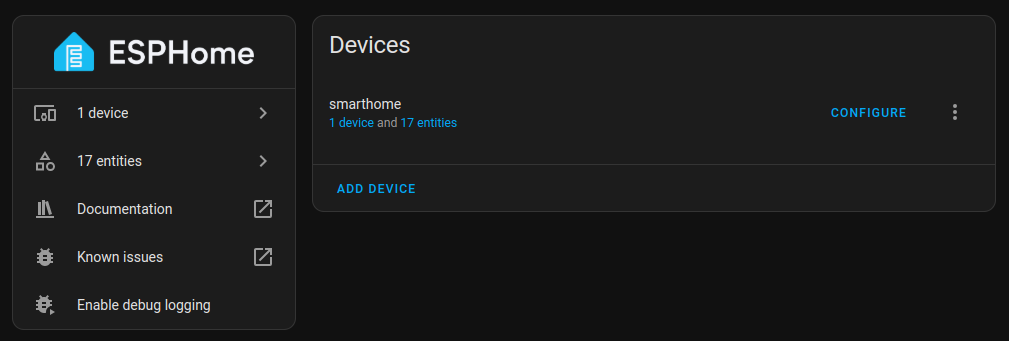
\includegraphics[width=140mm, keepaspectratio]{figures/homeassistant_esphome_int.png}
  \caption{ESPHome integration for Home Assistant set up}
  \label{fig:HAesphomeint}
\end{figure}

After successfully flashing the compiled firmware to the microcontroller, it can then be added to the Home Assistant environment with an "integration". Integration is a term in Home Assistant's ecosystem to connect and integrate other software and hardware platforms, in our case ESPHome to the Home Assistant environment as a device. \cite{HAConceptsTerminology}

\begin{lstlisting}[language=,caption=ESPHome configuration for a simple LED switch,label=lst:ESPHomeDevConf]
switch:
- platform: gpio
  id: bedroom_led
  pin:
    number: GPIO21
    mode: OUTPUT
  name: "BedroomLED"
  restore_mode: ALWAYS_OFF
\end{lstlisting}

ESPHome supports many types of electronic components connected to the microcontroller's pins (as the project's homepage shows), with a relatively easy configuration. \cite{ESPHomeHomepage} To set devices up to be utilized by ESPHome, their configuration has to be defined in the YAML configuration file, as shown in listing \ref{lst:ESPHomeDevConf} for a switch, that toggles an LED. Each device should have an \verb+id+ and \verb+name+ set, along with platform specific details, such as the GPIO pin number and mode (input / output).

This configuration was also done iteratively to the other connected components as well, but in separate files with the use of packages, which is a functionality provided by ESPHome for better code structuring and maintainability. \cite{ESPHomePackages} With packages, ESPHome configurations are merged from multiple YAML files to a single one during compilation, as if they were written in that single one.

\begin{lstlisting}[language=,caption=ESPHome package includes in the main configuration file,label=lst:ESPHomePackageIncludes]
packages:
  fans: !include packages/fans.yaml
  ldr: !include packages/ldr.yaml
  leds: !include packages/leds.yaml
  peltier: !include packages/peltier.yaml
  shutter: !include packages/shutter.yaml
  tempsensors: !include packages/tempsensors.yaml
\end{lstlisting}

\begin{figure}[!ht]
  \centering
  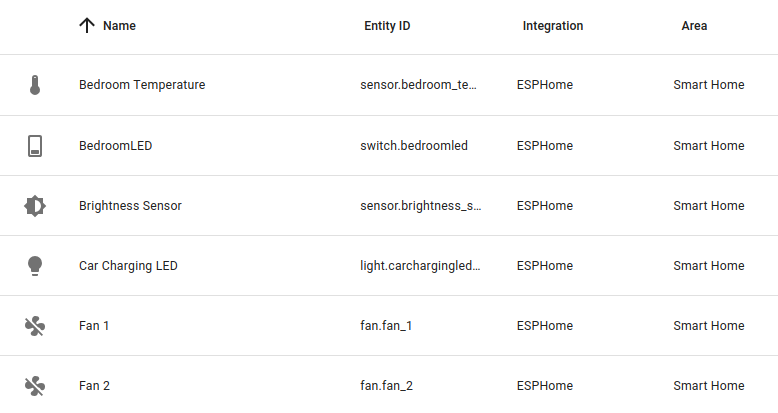
\includegraphics[width=150mm, keepaspectratio]{figures/esphome_entities.png}
  \caption{Home Assistant entities provided by the ESPHome integration}
  \label{fig:HAesphomeEntities}
\end{figure}

After reconfiguring the microcontroller with extra devices, Home Assistant automatically takes care of the devices added and new entities are created for them. In Home Assistant's terminology, entities are the basic building blocks that hold data and are used to monitor physical properties or control entities. \cite{HAConceptsTerminology} On \refstruc{fig:HAesphomeEntities}, a few entities from the ESPHome integration device are shown. 

\begin{figure}[!ht]
  \centering
  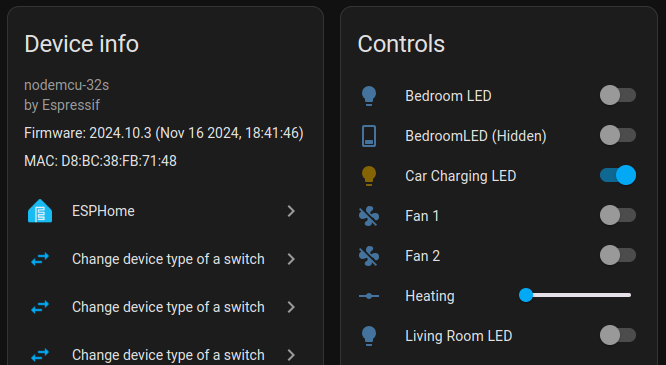
\includegraphics[width=150mm, keepaspectratio]{figures/esphome_controls.png}
  \caption{Device of the ESPHome integration and its control entities}
  \label{fig:HAesphomeControls}
\end{figure}

The ESPHome integration's device, its controls, sensors and configurations can also be seen and configured, as shown on \refstruc{fig:HAesphomeControls}.

One component connected to the microcontroller was harder to be configured for use, than others, which is the SG90 servo used for the rolling shutter. Fortunately, other ESPHome users had also tried to make this exact servo model work and one forum member was able to and provided configuration code for it, which includes PWM configuration, conversion of value from a number slider's -100 to 100 range to the servos 180 degrees of control and a sensor for the currently set position. \cite{ESPHomeForumSG90} This example superbly shows an advantage of open-source software and its communities, how projects can be easily extended with extra, more complex components and how users can get support for their problems.

\subsection{Additional user interface setup, customization}

\subsubsection{Entity customization}

\begin{figure}[!ht]
  \centering
  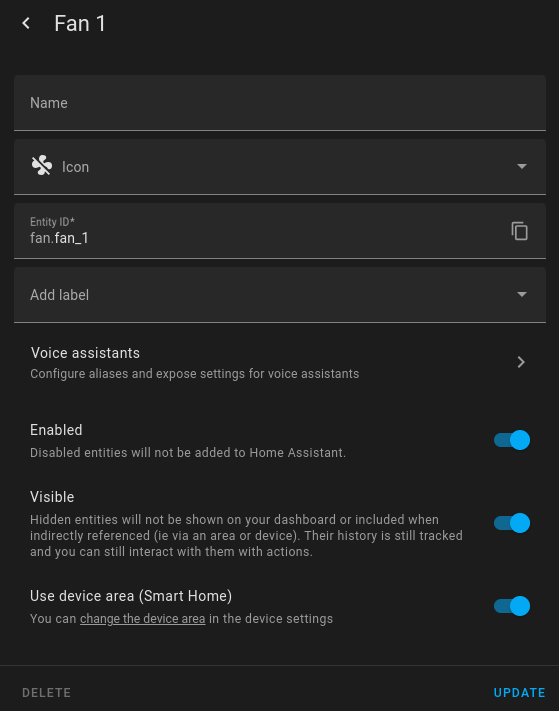
\includegraphics[width=90mm, keepaspectratio]{figures/homeassistant_entity_customization.png}
  \caption{Entity customization in Home Assistant}
  \label{fig:HAentityCustomization}
\end{figure}

Customizations can be applied on Home Assistant entities to better suit the user's needs. Each entity has a unique id, which is used as a basis to uniquely identify a specific entity and it is guaranteed to be static and never changes. \cite{HAFAQUniqueID} When present, it gets assigned an entity id, which is in the form of \verb+<domain>.<id>+ and is used as a logical identifier in dashboards, automations and others. \cite{HAEntitiesDomains} To give examples, \verb+fan.fan_1+ is in the \verb+fan+ domain, therefore can be controlled as a fan, has an id of \verb+fan_1+ and \verb+light.bedroom_led+ is a light with an id of \verb+bedroom_led+. The entity id can be changed if desired, but it has to be unique throughout the Home Assistant environment. And finally, each entity has a \verb+name+, which is used as a display name and is displayed on dashboards, can be referred to in the voice assistant, etc. Besides a name and id, an icon and labels can also be specified, as shown on \refstruc{fig:HAentityCustomization}.

\begin{figure}[!ht]
  \centering
  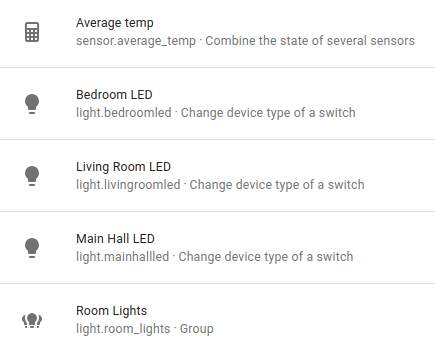
\includegraphics[width=110mm, keepaspectratio]{figures/homeassistant_helpers.png}
  \caption{Home Assistant helpers used in the project}
  \label{fig:HAhelpers}
\end{figure}

Helpers are software tools to add or change functionality of different entities. For example, the states of multiple devices can be combined to a single value (eg. to calculate the average temperature in the house), change the type of a switch to a different device (eg. togglable binary light, fan, lock) or combine multiple entities into a single virtual entity with the usage of the group feature. On \refstruc{fig:HAhelpers}, the helpers used in the project are shown.

\subsubsection{Dashboard customization}

Multiple dashboards can be created in Home Assistant to control and show different aspects and devices of a house. Upon setup, a default dashboard is automatically created, the layout of which is shown on \refstruc{fig:HAdefaultDashboard}.

\begin{figure}[!ht]
  \centering
  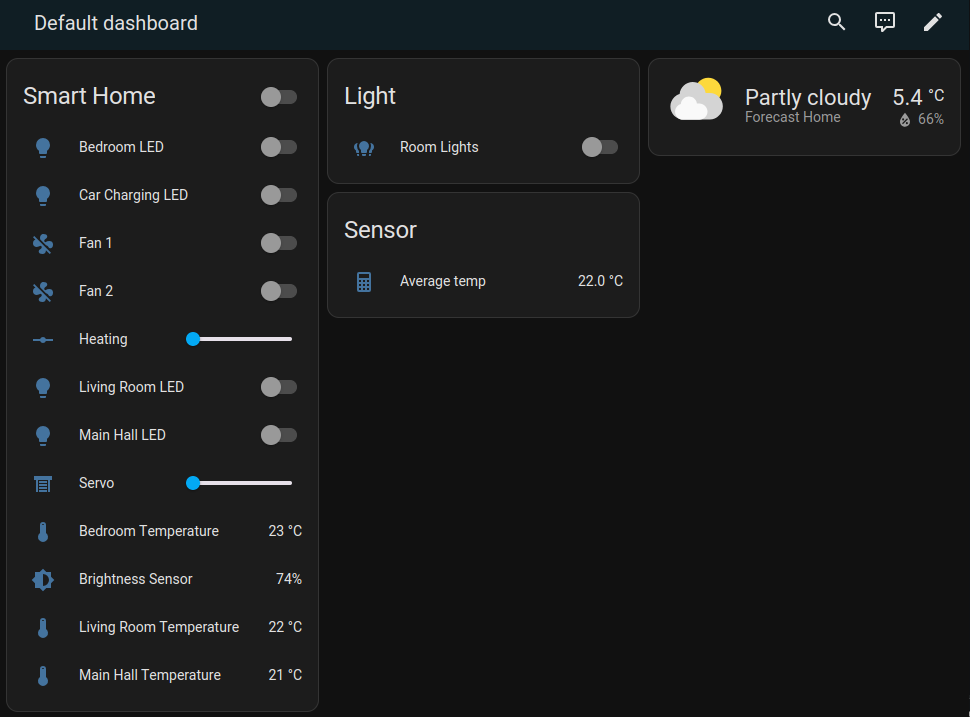
\includegraphics[width=150mm, keepaspectratio]{figures/homeassistant_dashboard_default.png}
  \caption{Default dashboard layout with controls and readings for the box device and weather forecast integration set to Budapest}
  \label{fig:HAdefaultDashboard}
\end{figure}

\begin{figure}[!ht]
  \centering
  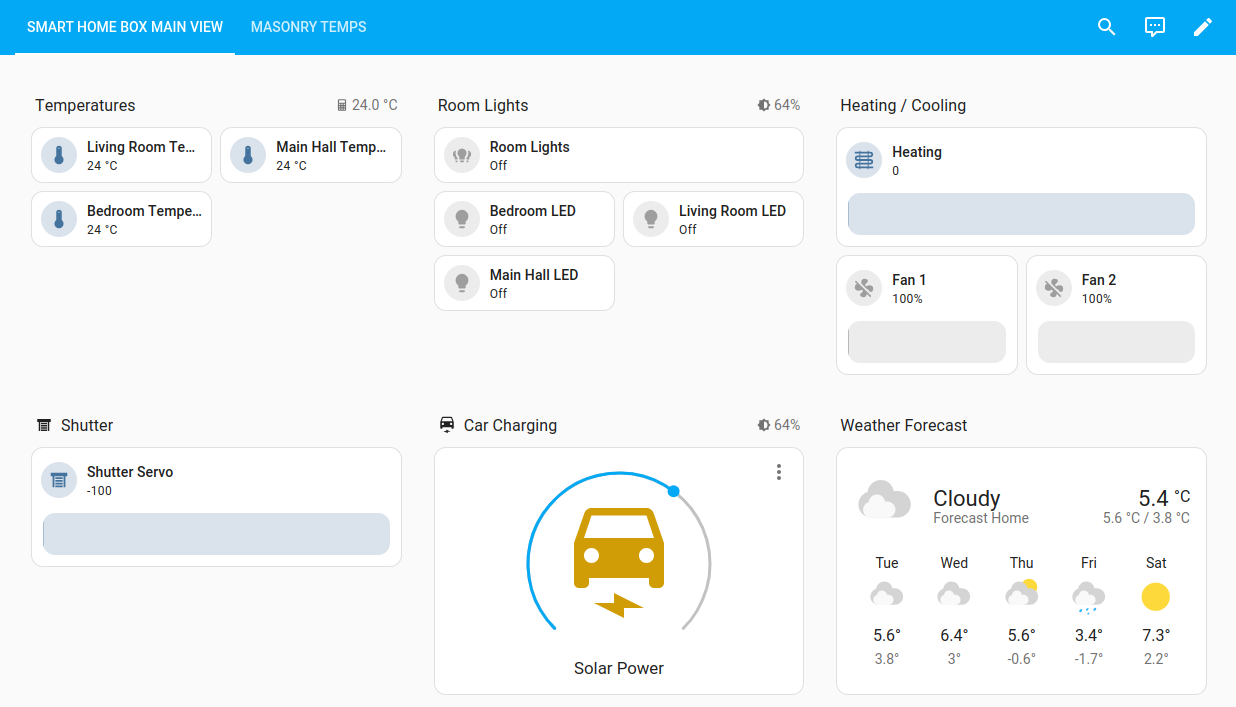
\includegraphics[width=150mm, keepaspectratio]{figures/homeassistant_dashboard_custom.png}
  \caption{Custom sections dashboard with devices grouped together by type and weather forecast integration set to Budapest}
  \label{fig:HAcustomDashboard}
\end{figure}

\begin{figure}[!ht]
  \centering
  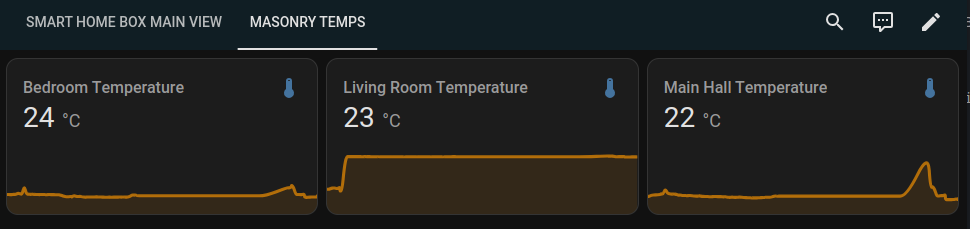
\includegraphics[width=150mm, keepaspectratio]{figures/homeassistant_dashboard_masonry.png}
  \caption{Masonry dashboard layout with historical graphs for room temperatures}
  \label{fig:HAmasonryDashboard}
\end{figure}

On the default dashboard, all areas, device controls and readings, integrations are shown as a whole, which can be ideal for a typical home environment with multiple devices, but not for the project with basically a single device and its many entities. Therefore another dashboard with a sections type view was created, which is shown on \refstruc{fig:HAcustomDashboard}. Multiple sections were created for the various types of controls (eg. lights, fans) and sensors (room temperatures), which were grouped together by the types of entities. Additional extra entities were added three sections for display: the average temperature of the three rooms to the "Temperatures" section and the LDR sensor's value to the "Room Lights" and "Car Charging" sections. The car charging section mimics electric car charging with imaginary solar panels (actually based on the value of the LDR): the set brightness of the automated LED is used as the value for display, click events on the section were disabled to make it read-only (from this dashboard).
% maybe areas, labels, zones(osm)?

A masonry type view was also added to the dashboard, which is shown on \refstruc{fig:HAmasonryDashboard}. When multiple views are present for a dashboard, a tab strip is shown to select between them, as shown on the screenshot. On the masonry view, added cards are sorted in columns based on their sizes, three equal sized historical graphs were added of the room temperatures recorded.

\subsection{Smartphone setup}

Besides having a web-based UI, Home Assistant also has mobile applications for the Android and iOS platforms called Home Assistant Companion. \cite{HACompanion} To test the mobile application, it was installed to a personal Android smartphone. The smartphone was connected to the Wi-Fi network with its credentials, and the IP address of the HA OS VM Wi-Fi adapter with the proper protocol and port (\verb+http://192.168.1.100:8123+) was entered into the application as the instance URL. On \refstruc{fig:HAandroidScreenshot}, a screenshot of the Android application is shown.

\begin{figure}[!ht]
  \centering
  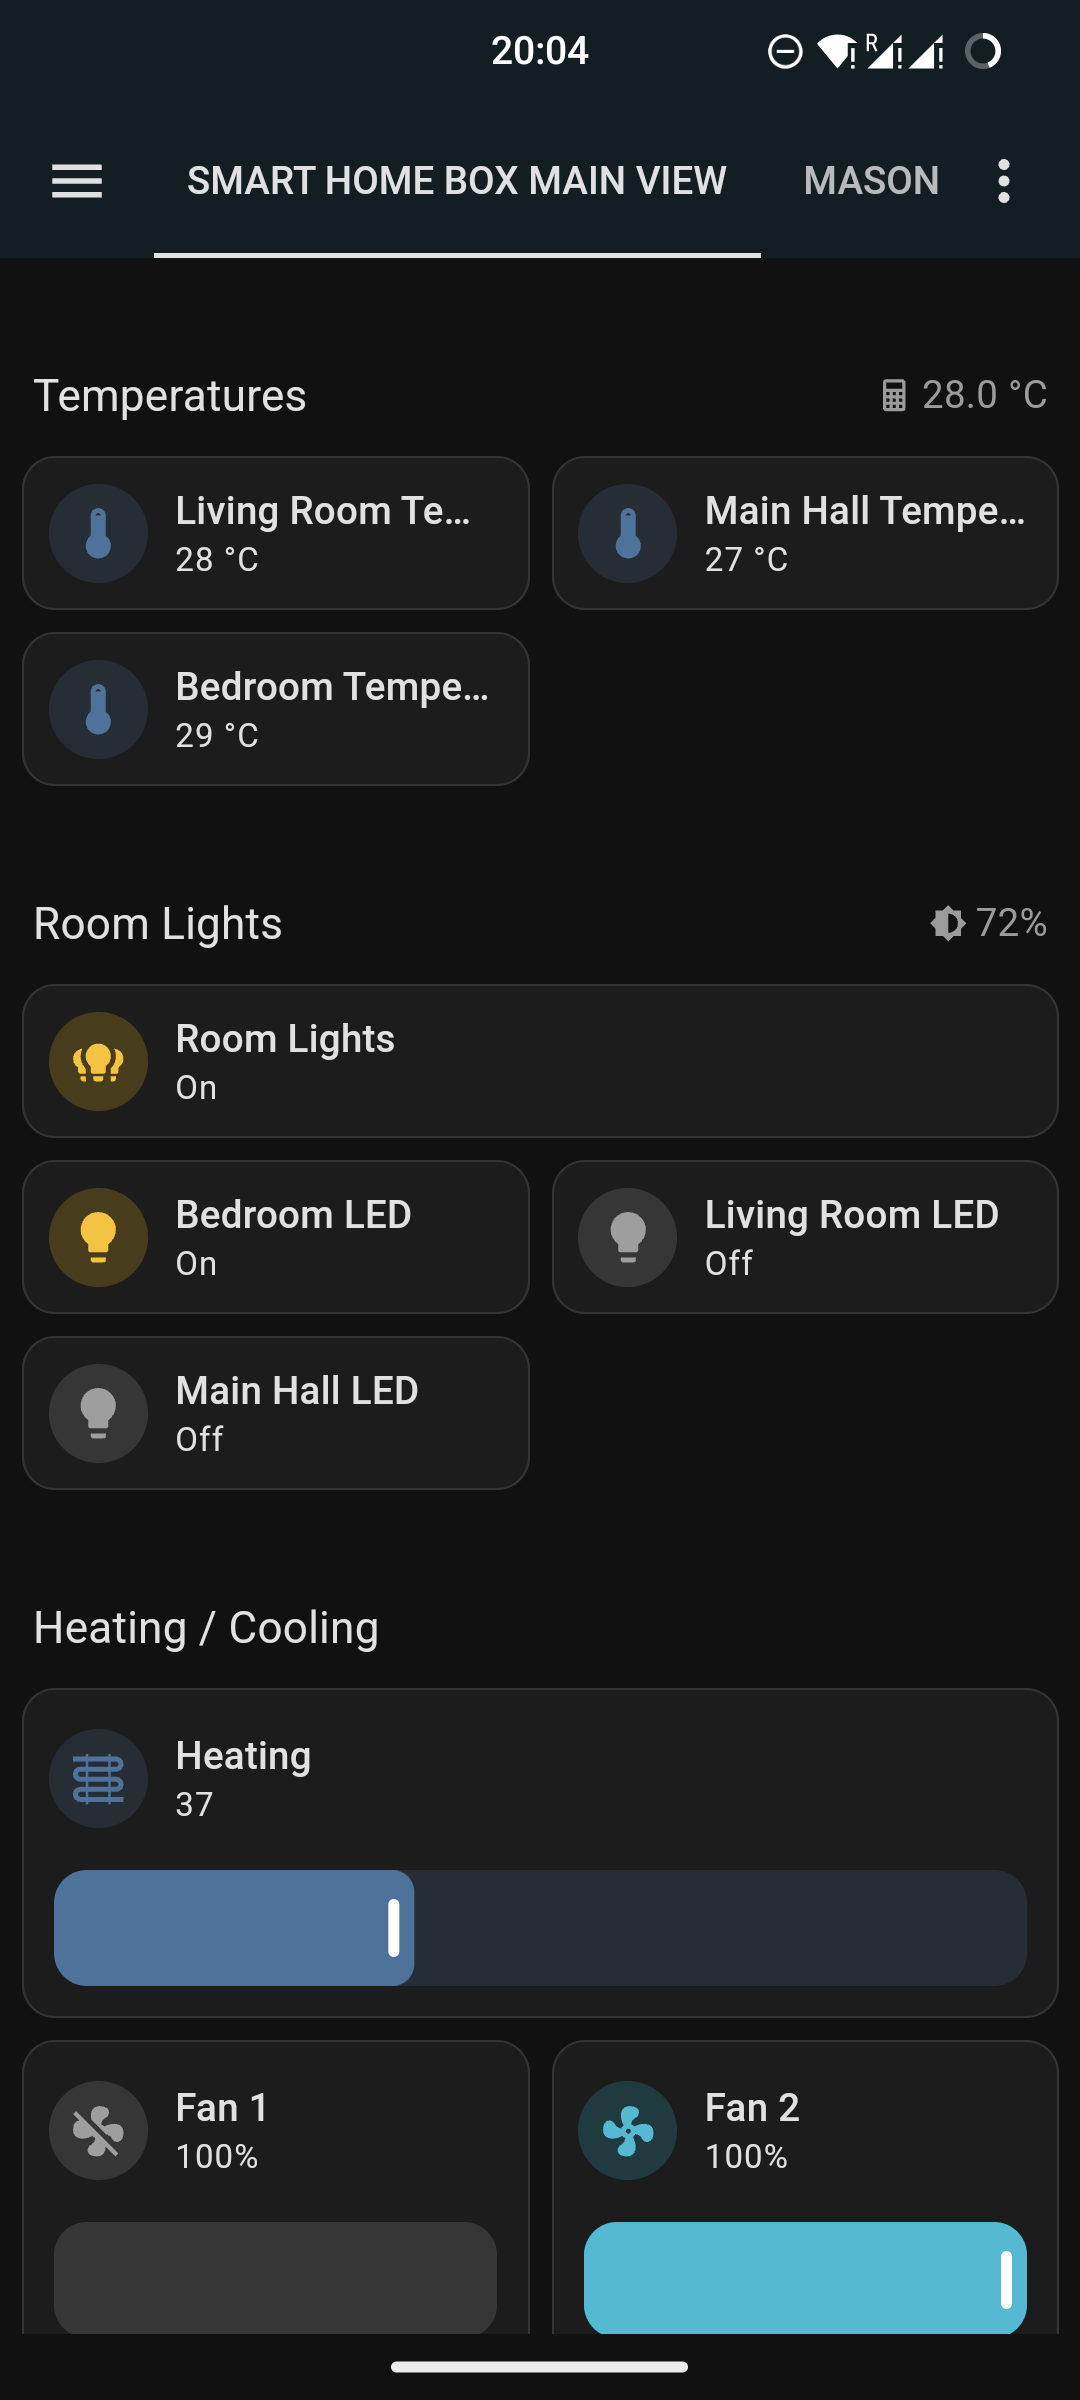
\includegraphics[width=70mm, keepaspectratio]{figures/homeassistant_android_screenshot.png}
  \caption{Home Assistant Companion app running on Android 14}
  \label{fig:HAandroidScreenshot}
\end{figure}

Contrary to expectations, simultaneous use of the the Internet-less Wi-Fi network and the phone's data-enabled SIM card for Internet connection didn't work, even if the "Mobile data always active" option was turned on in the developer settings. A message is shown when connecting to the network about it not having an Internet connection and whether the phone should stay connected to it and only upon pressing yes, can the server be reached. But at the same time, the status bar shows that LTE disappears, which can mean that the radio data connection is dropped or only the routing table is changed, but in such a way that the default gateway gets overriden to the Wi-Fi network. It would likely be possible to be able to change this behavior with a rooted phone (where a root shell access is present), but its risks and disadvantages aren't worth it for this simple test scenario. And in a typical home network environment, where there wouldn't be a need to access two networks simultaneously, the HA OS server and the Internet would be able to be reached at the same time.

\subsection{Automations}

To make the life of its users easier and more comfortable, Home Assistant offers automations to run specific tasks. An automation comprises of three parts: triggers (when it runs), conditions (optional, only run if these conditions are met) and actions (what actions to perform). \cite{HAAutomationBasics} Besides basic automations, there are further features closely related to them: scenes can be used to set a group of entities to a specified state, scripts can contain multiple actions and blueprints can be used to specify a generic automation framework, which can be used as a common basis for multiple different automations with exactly specified entities.

During Project Laboratory, one feature that the model box had is the ability to show "solar power" by changing the brightness of the LED put inside a toy car based on the readings of the LDR. This was possible to replicate in Home Assistant too, with the use of an automation. Two kinds of triggers were tried for detecting when the automation should run: the first was using "Brightness Sensor voltage change", however even with a very small duration specified (1-5 seconds) between 0 \% and 100\% set as the voltage percent range, the automation wasn't triggered frequently enough, only about once a minute. Therefore an other trigger was used: a periodic interval of 5 seconds, which works reliably and its configuration is shown on \refstruc{fig:HAautomationTrigger}.

\begin{figure}[!ht]
  \centering
  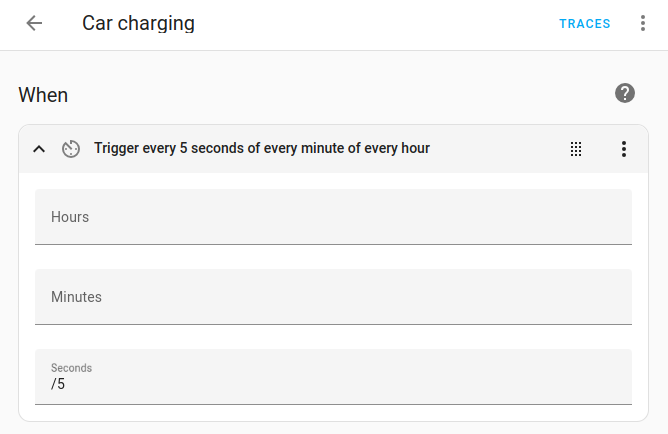
\includegraphics[width=110mm, keepaspectratio]{figures/homeassistant_automation_trigger.png}
  \caption{Home Assistant automation trigger}
  \label{fig:HAautomationTrigger}
\end{figure}

The action needed to accomplish one simple task: set the brightness value of the car charging LED, based on the readings of the LDR. This was possible to be defined via the YAML editor (the set content is shown in listing \ref{lst:HAautomationAction}), as the visual editor would have only allowed a constant number to be set as brightness. For action, \verb+light.turn_on+ was specified, that turns on the specified target light entity (which is \verb+light.car_carging_led+, if it isn't on already) and a \verb+brightness_pct+ data key is also specified, which tells \verb+light.turn_on+ what the target light's brightness should be set to. This key is defined to be the result of a template (inside double curly braces): \verb+states()+ retrieves the value of the LDR reading, which is in the form of an integer between 0 and 100 and it gets set to be \verb+brightness_pct+.

\begin{lstlisting}[language=,caption=Home Assistant automation action for setting LED brightness based on LDR,label=lst:HAautomationAction]
action: light.turn_on
metadata: {}
data:
  brightness_pct: "{{ states('sensor.brightness_sensor') }}"
target:
  entity_id: light.car_carging_led  
\end{lstlisting}
\newpage
\subsection{Voice assistant}

As a prerequisite for the locally hosted voice assistant, the Home Assistant Docker environment was migrated to HA OS running in a VM, explained with more details in chapter 3.4.1. To set up the voice assistant environment, the installation guide was followed to set up the Piper (text-to-speech) and Whisper (speech-to-text) add-ons. \cite{HALocalAssist} The add-ons were configured to use a low quality speech detection and synthetization, in order to ensure fast response, as even with medium, the response time dramatically increased after pronouncing the commands. A screenshot of the assistant can be seen on \refstruc{fig:HAandroidVoiceAssistant}. The speech detection and synthetization supports many languages to be configured: English (UK, US), German and Hungarian were tried and out of these, English had the best accuracy of understanding and executing the said commands. Although it is impressive, it only works with simple commands, when exact device names are specified and doesn't reach the level of Artificial Intelligence based chatbots, that gained a rapid technology boom in the last few years.

\begin{figure}[!ht]
  \centering
  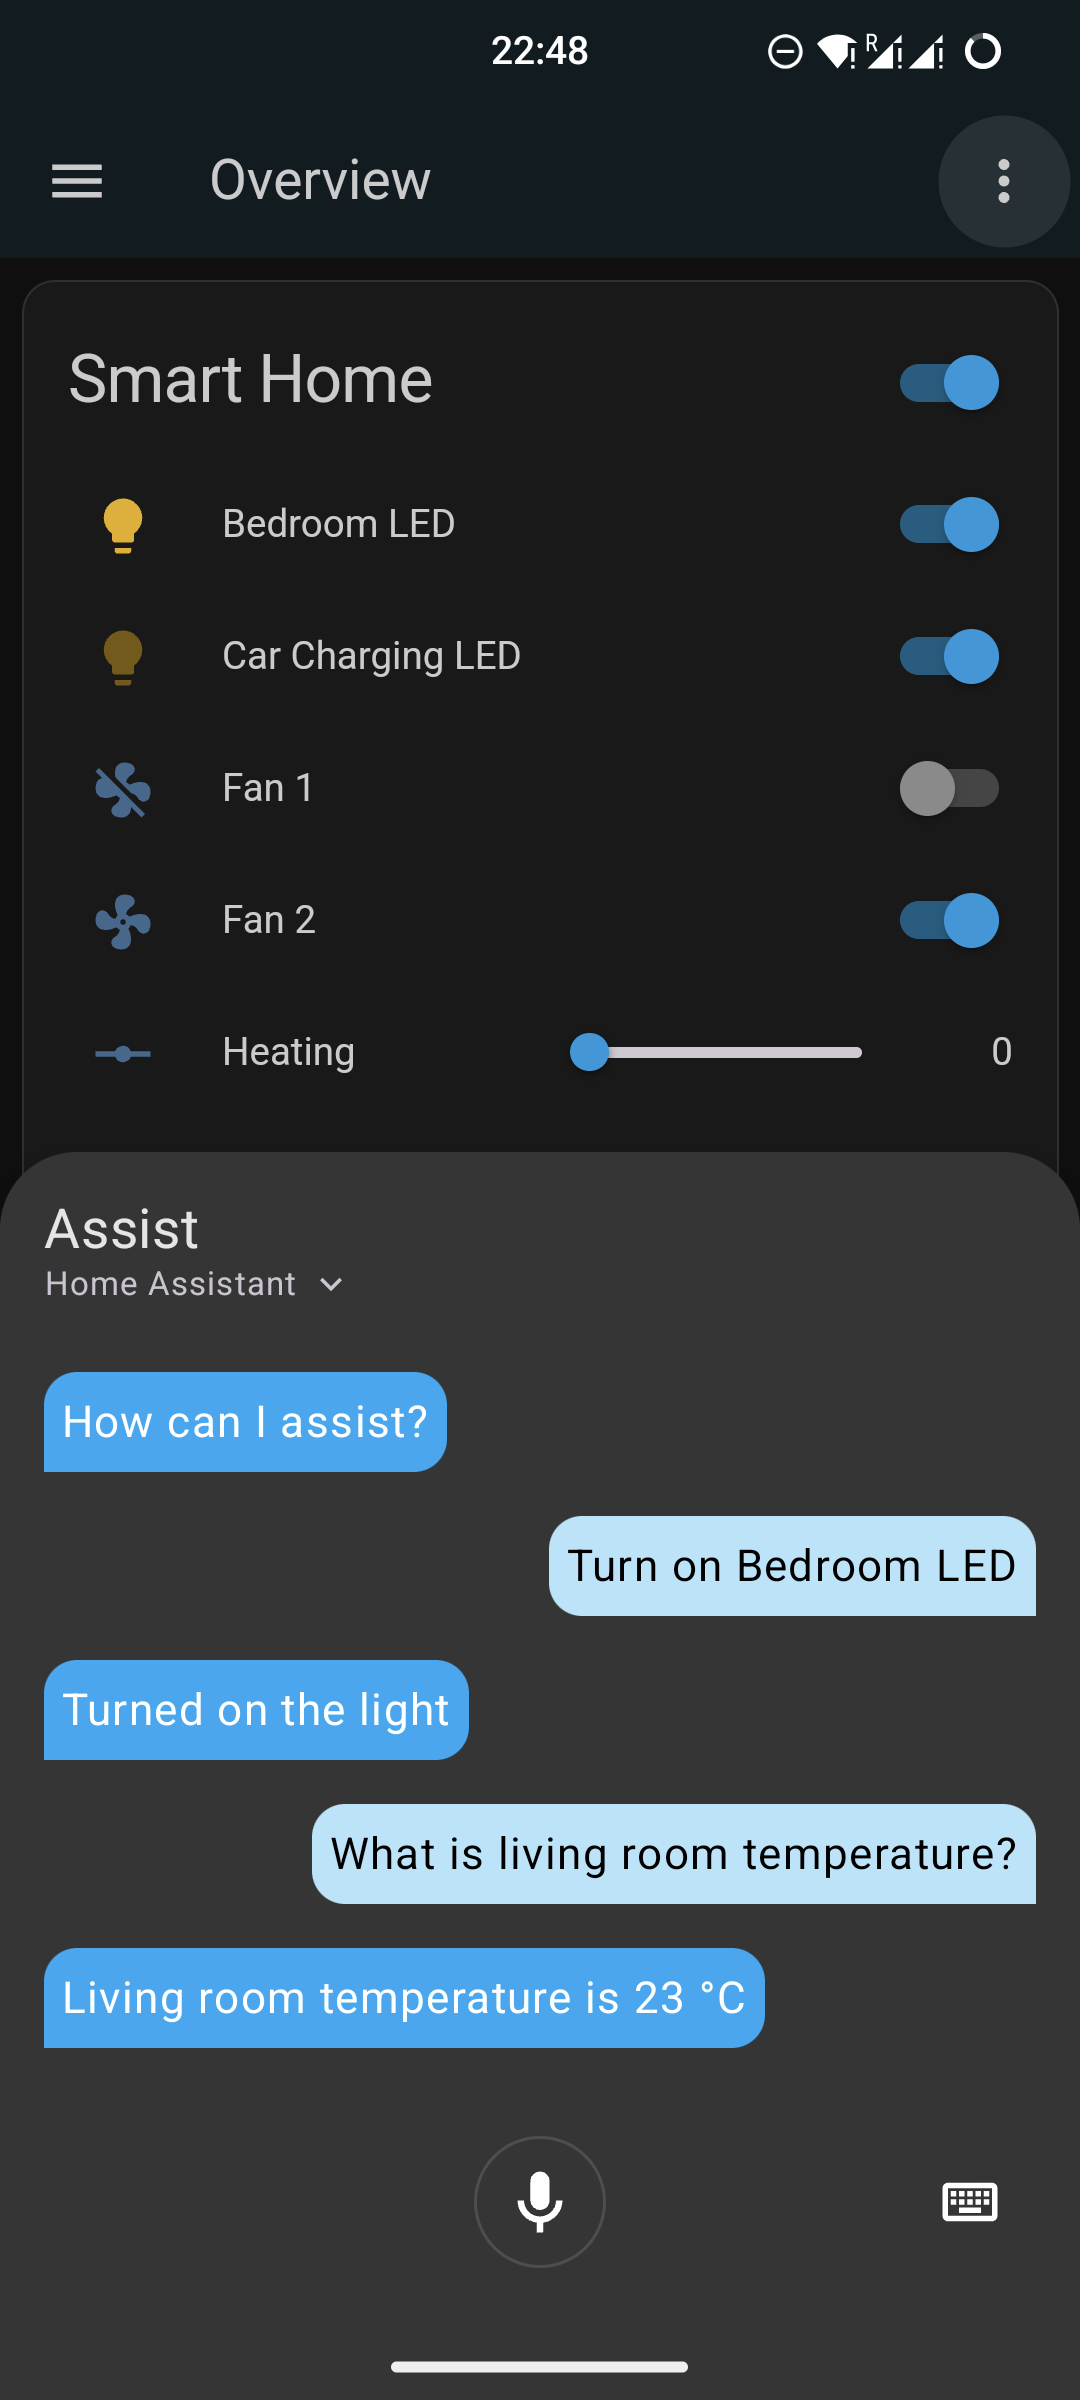
\includegraphics[width=68mm, keepaspectratio]{figures/homeassistant_android_assist.png}
  \caption{Screenshot of Home Assistant's locally hosted voice assistant in action}
  \label{fig:HAandroidVoiceAssistant}
\end{figure}
